% Originally: content/week-11.tex, \subsection{The Poincare lemma and simply connected domains} --- promoted

\section{The Poincaré lemma and simply connected domains}
\label{sec:poincare_lemma_simply_connected}

% Transition: Claude Opus 5.5 (Extra)
\Cref{lem:integrability_conditions} gives a necessary condition for a potential. When is it also
sufficient? \Cref{prop:work_difference_potential} points the way: a potential exists as soon as
the integral of $F$ along a path depends only on the path's endpoints, for then
$f(x) := \int_{x_0}^{x} F$ is well defined. The question becomes when two paths with the same
endpoints give the same integral. For a field satisfying the integrability conditions, which in
the language of \cref{ch:differential_forms} says that the $1$-form
$\alpha = \sum_k F_k\,dx^k$ is closed, the answer is: whenever one path can be deformed into the
other.

% Transcribed content resumes here (provenance: the % Originally: line at the top of this file).
\begin{theorem}[Poincaré Lemma]
\label{thm:poincare_lemma}
Let $U \subseteq \mathbb{R}^n$ be open, and let $\alpha \in \Omega^1(U)$ be a $C^1$ closed $1$-form, that is, $d\alpha = 0$.
Let $\gamma_0, \gamma_1 : [0,1] \to U$ be piecewise $C^1$ paths with the same initial point $x_0$ and the same endpoint $x_1$. Suppose that $\gamma_0$ and $\gamma_1$ are \newterm{homotopic} in $U$ with fixed endpoints. For simplicity, assume that the homotopy $H : [0,1]^2 \to U$ is smooth. Then
\[\int_{\gamma_0} \alpha = \int_{\gamma_1} \alpha.\]
\end{theorem}

% Generator: Claude Opus 5.5 (Extra) --- proof added for self-containedness. With a smooth homotopy
% it is four lines: closedness of alpha, pulled back to the square, says that the integral along
% the intermediate paths has derivative equal to a boundary term, and the fixed endpoints kill it.
\begin{proof}
Write $H(s,\cdot)$ for the intermediate paths, so that $H(0,\cdot) = \gamma_0$ and
$H(1,\cdot) = \gamma_1$, and pull $\alpha$ back to the square (\cref{def:pullback_of_forms}):
\[H^*\alpha = P\,ds + Q\,dt, \qquad P := \alpha_H(\partial_sH), \quad Q := \alpha_H(\partial_tH).\]
The pullback commutes with $d$, so
$(\partial_sQ - \partial_tP)\,ds\wedge dt = d(H^*\alpha) = H^*(d\alpha) = 0$, that is,
$\partial_sQ = \partial_tP$. Now $I(s) := \int_0^1 Q(s,t)\,dt$ is the integral of $\alpha$ along
the path $H(s,\cdot)$, so the claim is $I(0) = I(1)$. Differentiating under the integral sign
(\cref{thm:feynmans_trick}),
\[I'(s) = \int_0^1 \partial_sQ(s,t)\,dt = \int_0^1 \partial_tP(s,t)\,dt = P(s,1) - P(s,0).\]
Both terms vanish, because the endpoints are fixed: $H(s,0) = x_0$ and $H(s,1) = x_1$ for every
$s$, so $\partial_sH = 0$ at $t = 0$ and at $t = 1$. Hence $I$ is constant.
\end{proof}

The proof shows what \qt{closed} means geometrically. Deforming the path changes the integral
only through what happens at its ends, and with the ends pinned there is nothing left to change.

\begin{corollary}[Existence of potentials in simply connected domains]
\label{cor:potentials_simply_connected}
Let $U \subseteq \mathbb{R}^n$ be an open \newterm{simply connected} set. Then every closed $C^1$ $1$-form on $U$ is exact. That is, if $\alpha \in \Omega^1(U)$ satisfies $d\alpha = 0$, then there exists a function $f \in C^2(U)$ such that $\alpha = df$.
Equivalently, if $F \in C^1(U, \mathbb{R}^n)$ satisfies the integrability conditions
\[\partial_j F_k = \partial_k F_j \qquad \text{for all } j, k \in \{1,\dots,n\},\]
then $F$ is conservative: there exists a potential $f \in C^2(U)$ such that $\nabla f = F$.
\end{corollary}

% Correction: Claude Opus 5 (High) --- this note used to state the definition of "simply connected"
% informally, which was the document's only account of the term although chapters 7 and 8 already
% used it. The definition now lives at def:simply_connected in 08-connectedness, taken from the
% script's 14.41; what remains here is the intuition and the list of examples, which is what the
% note was actually good for. Keep the two in step.
\begin{ainote}[Intuition on simply connected spaces]
Recall from \cref{def:simply_connected} that $U$ is simply connected when any two paths in $U$ with
the same endpoints are homotopic, or equivalently (\cref{rem:homotopy_as_deformation}) when any
closed loop in $U$ can be continuously contracted to a point within $U$.

% Supplement: Sascha Brack/Class Notes/Week_12_Notes_Monday.pdf, p. 7
\begin{center}
% Correction: Claude Opus 5 (High) --- five nested arcs, and every label sat in a GAP between
% two of them (`above' for the top two, `below' for the rest), so no label was attached to the
% arc it names: gamma_{0.25} read as labelling gamma_0's arc from underneath, and the gamma_1
% arc printed straight through the word gamma_{0.75}. Each label now sits ON its own arc with
% the white plate from style.md, which both breaks the line it belongs to -- the standard way
% to name a family of curves -- and stops any other arc printing through it.
%
% The floating $H(0,\cdot) = \gamma_0$ off at (-0.5,0.5) named nothing in particular and
% duplicated the gamma_0 already on the arc. Folded into that arc's own label, which makes it
% symmetric with the $\gamma_1 = H(1,\cdot)$ the bottom arc already carried.
% Note the plate here is fully opaque, unlike the softened one style.md gives for labels over a
% shaded region. What sits behind these labels is a `thick' black arc, and at 0.85 the remaining
% 15% printed as a clear grey stroke across the glyphs -- exactly the mud the plate is meant to
% prevent. A clean break in the line is also how a contour is normally named.
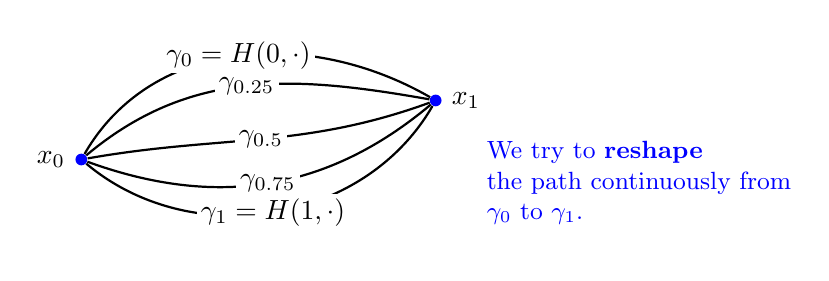
\begin{tikzpicture}[scale=1.5,
  lbl/.style={fill=white, text opacity=1, inner sep=1.5pt}]
  \node[circle, fill=blue, inner sep=1.5pt, label=left:{$x_0$}] (x0) at (0,0) {};
  \node[circle, fill=blue, inner sep=1.5pt, label=right:{$x_1$}] (x1) at (3,0.5) {};

  \draw[thick] (x0) to[out=60, in=150] node[lbl, pos=0.5] {$\gamma_0 = H(0,\cdot)$} (x1);
  \draw[thick] (x0) to[out=40, in=170] node[lbl, pos=0.5] {$\gamma_{0.25}$} (x1);
  \draw[thick] (x0) to[out=10, in=200] node[lbl, pos=0.5] {$\gamma_{0.5}$} (x1);
  \draw[thick] (x0) to[out=-20, in=220] node[lbl, pos=0.5] {$\gamma_{0.75}$} (x1);
  \draw[thick] (x0) to[out=-40, in=240] node[lbl, pos=0.5] {$\gamma_1 = H(1,\cdot)$} (x1);

  \node[blue, align=left, font=\small, anchor=west] at (3.35, -0.2) {We try to \textbf{reshape}\\the path continuously from\\$\gamma_0$ to $\gamma_1$.};
\end{tikzpicture}
\end{center}

Examples of simply connected spaces:
\begin{itemize}
    \item $\mathbb{R}^n$
    \item $\mathbb{R}^3 \setminus \{(0,0,0)\}$
\end{itemize}
Examples of spaces that are \emph{not} simply connected:
\begin{itemize}
    \item $S^1 \subseteq \mathbb{R}^2$ (the unit circle)
    \item $\mathbb{R}^3 \setminus \operatorname{span}\{(0,0,1)\transp\}$ (the $z$-axis removed)
    \item The torus
\end{itemize}
This topological property is what allows the integrability conditions to globally imply the existence of a potential.
\end{ainote}

% Generator: Claude Opus 5.5 (Extra) --- proof added for self-containedness. It is the
% construction every potential computation in this chapter performs by hand: integrate from a
% base point, and use the Poincare lemma to know the answer does not depend on the route.
\begin{proof}[Proof of \cref{cor:potentials_simply_connected}]
Write $\alpha = \sum_i F_i\,dx_i$, so that $\int_\gamma\alpha = \int_\gamma F\cdot d\gamma$ and
$d\alpha = 0$ is exactly the integrability condition. Fix a base point $x_0 \in U$.

\textbf{Polygonal paths reach everything.} Run the proof of
\cref{prop:open_euclidean_connected_path_connected} with \qt{polygonal path} (finitely many
straight segments, traversed one after another) in place of \qt{path}. Every step survives: the
constant path is polygonal, and the only paths the argument appends are straight segments inside a
ball. So in a connected open set any two points are joined by a polygonal path, which is piecewise
$C^1$. As $U$ is path-connected, hence connected, every $x \in U$ is reached from $x_0$ by such a
path $\gamma_x$.

\textbf{The candidate potential is well defined.} Put
\[f(x) := \int_{\gamma_x}\alpha .\]
Any two piecewise $C^1$ paths from $x_0$ to $x$ are homotopic with fixed endpoints, because $U$ is
simply connected, so by \cref{thm:poincare_lemma} they give the same integral, and $f(x)$ does not
depend on which $\gamma_x$ was chosen. (The lemma as stated assumes a smooth homotopy. That a
continuous homotopy between piecewise $C^1$ paths can be smoothed without leaving the open set $U$
is a standard approximation fact, which we use without proof.)

\textbf{Its gradient is $F$.} Let $x \in U$, $B_r(x) \subseteq U$, $i \in \{1,\dots,n\}$ and
$0 < \lvert t\rvert < r$. A path from $x_0$ to $x+te_i$ is $\gamma_x$ followed by the segment
$\sigma(s) := x + s\,te_i$, $s \in [0,1]$, which stays in the ball. Since the integral over a
concatenation is the sum of the integrals (\cref{ex:path_concatenation_work}),
\[f(x+te_i) - f(x) = \int_\sigma F\cdot d\sigma = \int_0^1 F_i(x+ste_i)\,t\,ds
  = \int_0^t F_i(x+ue_i)\,du .\]
Dividing by $t$ and letting $t \to 0$, the fundamental theorem of calculus gives
$\partial_if(x) = F_i(x)$. Hence $\nabla f = F$, which is $C^1$, so $f \in C^2(U)$ and
$df = \alpha$.
\end{proof}

% Generator: Claude Opus 5.5 (Extra) --- the route in the proof above. x_0 = (0,0), x = (3,1);
% gamma_x is a three-segment polygon (0,0) -> (1.2,1.3) -> (2.1,0.2) -> (3,1). The step to
% x + t e_1 = (3.8,1) is horizontal, inside the dashed ball B_r(x) of radius 0.95, which is all
% the proof differentiates. A second, curved route from x_0 to x (dashed) is drawn to show the
% choice of gamma_x does not matter, which is the Poincare lemma's contribution.
\begin{center}
\begin{tikzpicture}[>=Latex, scale=1.15,
  lbl/.style={fill=white, fill opacity=0.85, text opacity=1, inner sep=1.2pt, rounded corners=1pt}]
  \draw[gray, dashed] (3,1) circle (0.95);
  \draw[->, thick, blue!70!black] (0,0) -- (1.2,1.3) -- (2.1,0.2) -- (2.96,0.96);
  \draw[thick, dashed, gray!70!black] (0,0) .. controls (0.6,-1.0) and (2.6,-0.9) .. (3,1);
  \draw[->, very thick, BurntOrange] (3,1) -- (3.8,1);
  \fill (0,0) circle (1.6pt) node[left] {$x_0$};
  \fill (3,1) circle (1.6pt);
  \node[lbl, above left] at (2.95,1.05) {$x$};
  \fill (3.8,1) circle (1.6pt) node[right] {$x+te_i$};
  \node[lbl, font=\small, text=blue!70!black] at (1.0,1.55) {$\gamma_x$};
  \node[lbl, font=\scriptsize, text=gray!60!black, align=center] at (1.6,-1.1)
    {another route:\\ same integral (Poincaré)};
  \node[lbl, font=\scriptsize, text=BurntOrange, below] at (3.45,0.92) {$\sigma$};
  \node[font=\scriptsize, text=gray] at (4.25,1.85) {$B_r(x)$};
\end{tikzpicture}
\end{center}

\begin{remark}[Computing a potential in practice]
\label{rem:potential_by_line_integral}
The proof is also a recipe. On a star-shaped $U$ take straight segments from the centre
$x_0$, so $f(x) = \int_0^1 F\big(x_0 + s(x-x_0)\big)\cdot(x-x_0)\,ds$; on a box, the staircase
of coordinate steps used in the proof of \cref{thm:continuous_partials_imply_differentiable} is
often quicker, since each step integrates a single component $F_i$ in a single variable.
\end{remark}

% Supplement: Analysis_II_Script_v1.pdf, p. 153
\begin{example}[Integrability without a potential: why simple connectedness is needed]
\label{ex:vortex_field_not_conservative}
Let $U := \mathbb{R}^2\setminus\{0\}$ (which is \emph{not} simply connected, unlike its
$3$-dimensional analogue $\mathbb{R}^3\setminus\{0\}$ listed above) and
\[F(x,y) := \left(\frac{-y}{x^2+y^2},\ \frac{x}{x^2+y^2}\right), \qquad (x,y) \in U.\]
A direct computation gives
\[\partial_1F_2 = \partial_x\!\left(\frac{x}{x^2+y^2}\right) = \frac{-x^2+y^2}{(x^2+y^2)^2}
  = \partial_y\!\left(\frac{-y}{x^2+y^2}\right) = \partial_2F_1,\]
so $F$ satisfies the integrability conditions (\cref{lem:integrability_conditions})
\emph{everywhere} on $U$. Yet $F$ is not conservative: for the loop
$\gamma(t) := (\cos(2\pi t),\sin(2\pi t))$, $t\in[0,1]$, tracing the unit circle once
counterclockwise,
\[\oint_\gamma F\cdot d\gamma
  = 2\pi\int_0^1\langle(-\sin(2\pi t),\cos(2\pi t)),(-\sin(2\pi t),\cos(2\pi t))\rangle\,dt
  = 2\pi \neq 0,\]
which by \cref{prop:work_difference_potential} is impossible for a conservative field (a closed
loop would have to return $f(\gamma(1))-f(\gamma(0))=0$). This is exactly the witness that
\cref{cor:potentials_simply_connected} needs the hypothesis it has: the integrability
conditions are necessary but, on a domain that is not simply connected, not sufficient.
\end{example}

% Source: old_exams/HS20.pdf (Analysis I & II, 27 January 2021, Prof. Peter S. Jossen),
% Teil B, Aufgabe 3, p. 20
% Extractor: Claude Opus 5 (High)
% Filed directly after ex:vortex_field_not_conservative because it is that example's mirror image,
% and the pair is the point: "not simply connected" is a reason the corollary DOES NOT APPLY, not a
% proof that the field fails to be conservative. Part (e) of the original, asking for the
% definition of a work integral, is omitted -- def:line_integral gives it.
\begin{exercise}[Integrability conditions on a domain that is not connected]
\label{ex:jossen_potential_on_disconnected_domain}
Let $g : \mathbb{R} \to \mathbb{R}$ be twice continuously differentiable and let $F$ be the vector
field defined on $U := \{(x,y,z) \in \mathbb{R}^3 : y \neq 0\}$ by
\[F(x,y,z) := \left((1+x)\,e^{x+\frac1y},\ \ -\frac{x}{y^2}\,e^{x+\frac1y},\ \ g'(z)\right).\]
\begin{enumerate}[label=\textbf{(\alph*)}]
  \item Is $U$ open? Is it connected? Is it simply connected?
  \item Does $F$ satisfy the integrability conditions?
  \item Is $F$ conservative? Justify your answer.
  \item Does $F$ admit a potential? If so, give one; if not, explain why not.
  \item Compute the work integral $\int_\gamma F \cdot d\gamma$ along the path
    $\gamma : [0,1] \to U$, $\gamma(t) := \big(t\cos(2\pi t),\ 2 + t\sin(2\pi t),\ t^2-t+1\big)$.
    Check first that $\gamma$ really does take values in $U$.
\end{enumerate}
\exinfo{This exercise is taken from the Analysis I \& II examination of 27 January 2021
(Prof.\ Peter S.\ Jossen), Part B, Problem 3, one part of which asks for the definition of a work
integral and is omitted here.}
\exsol{sol:jossen_potential_on_disconnected_domain}
\end{exercise}

% Source: old_exams/august2025.pdf (Prof. Laura Kobel-Keller), Analysis II examination,
% August 2025, Frage 9, printed p. 8
% Extractor: Claude Opus 5 (High)
\begin{exercise}[Single choice: what irrotational buys you, and what it does not]
\label{ex:kobel_irrotational_single_choice}
Let $V$ be an irrotational vector field on $G \subseteq \mathbb{R}^2$, that is, $\curl(V) = 0$
throughout $G$. Exactly one of the following is correct. Which?
\begin{enumerate}[label=\textbf{(\alph*)}]
  \item The line integral over any closed curve lying entirely in $G$ must be zero.
  \item If in addition $G$ is connected, then $V$ must have a potential: there must exist
    $\varphi(x,y)$ with $\nabla\varphi = V$ on all of $G$.
  \item It must also hold that $\divg(V) = 0$.
  \item It may be that there exists a potential $\varphi(x,y)$ on $G$ with $\nabla\varphi = V$.
\end{enumerate}
\exinfo{This exercise is taken from the Analysis II examination of August 2025
(Prof.\ Laura Kobel-Keller), Question 9.}
\exsol{sol:kobel_irrotational_single_choice}
\end{exercise}
